\section{External ILD integration}
%\writer{Yasuhiro Sugimoto}{1}
\label{ild:sec:external_integration}
%Generic layout of the cavern, mentioning the current options for its configuration (TDR, Tohoku, YS).

The proposed site for the ILC is located in the Kitakami mountains in the north of the Japanese main island Honshu. Dedicated studies are under way to adapt the generic ILC design, as described in the Technical Design Report, to the realities in this environment. For ILD, the arrangements of the surface and underground installations around the interaction point (IP) are of natural importance. The current conceptual design of the civil facilities and the plans for the detector related infrastructure and services have been coordinated between the relevant detector and ILC machine groups as well as with local experts.

\subsection{Site-related Infrastructure}

ILD is foreseen to be assembled on the surface, similar to CMS at LHC. Figure~\ref{fig:integration:surface} shows a rendering of the surface installations above the ILC interaction point. At the heart is the detector assembly building that is located directly over the central shaft that gives access to the underground collider hall. A large gantry crane above the shaft allows for the lowering of the pre-instrumented detector parts into the underground area. A preparation building is foreseen where sub-detector elements can be assembled and tested. A research building and a computing building provide the infrastructure for the operation of the detectors at the IP Campus. 

\begin{figure}[h!]
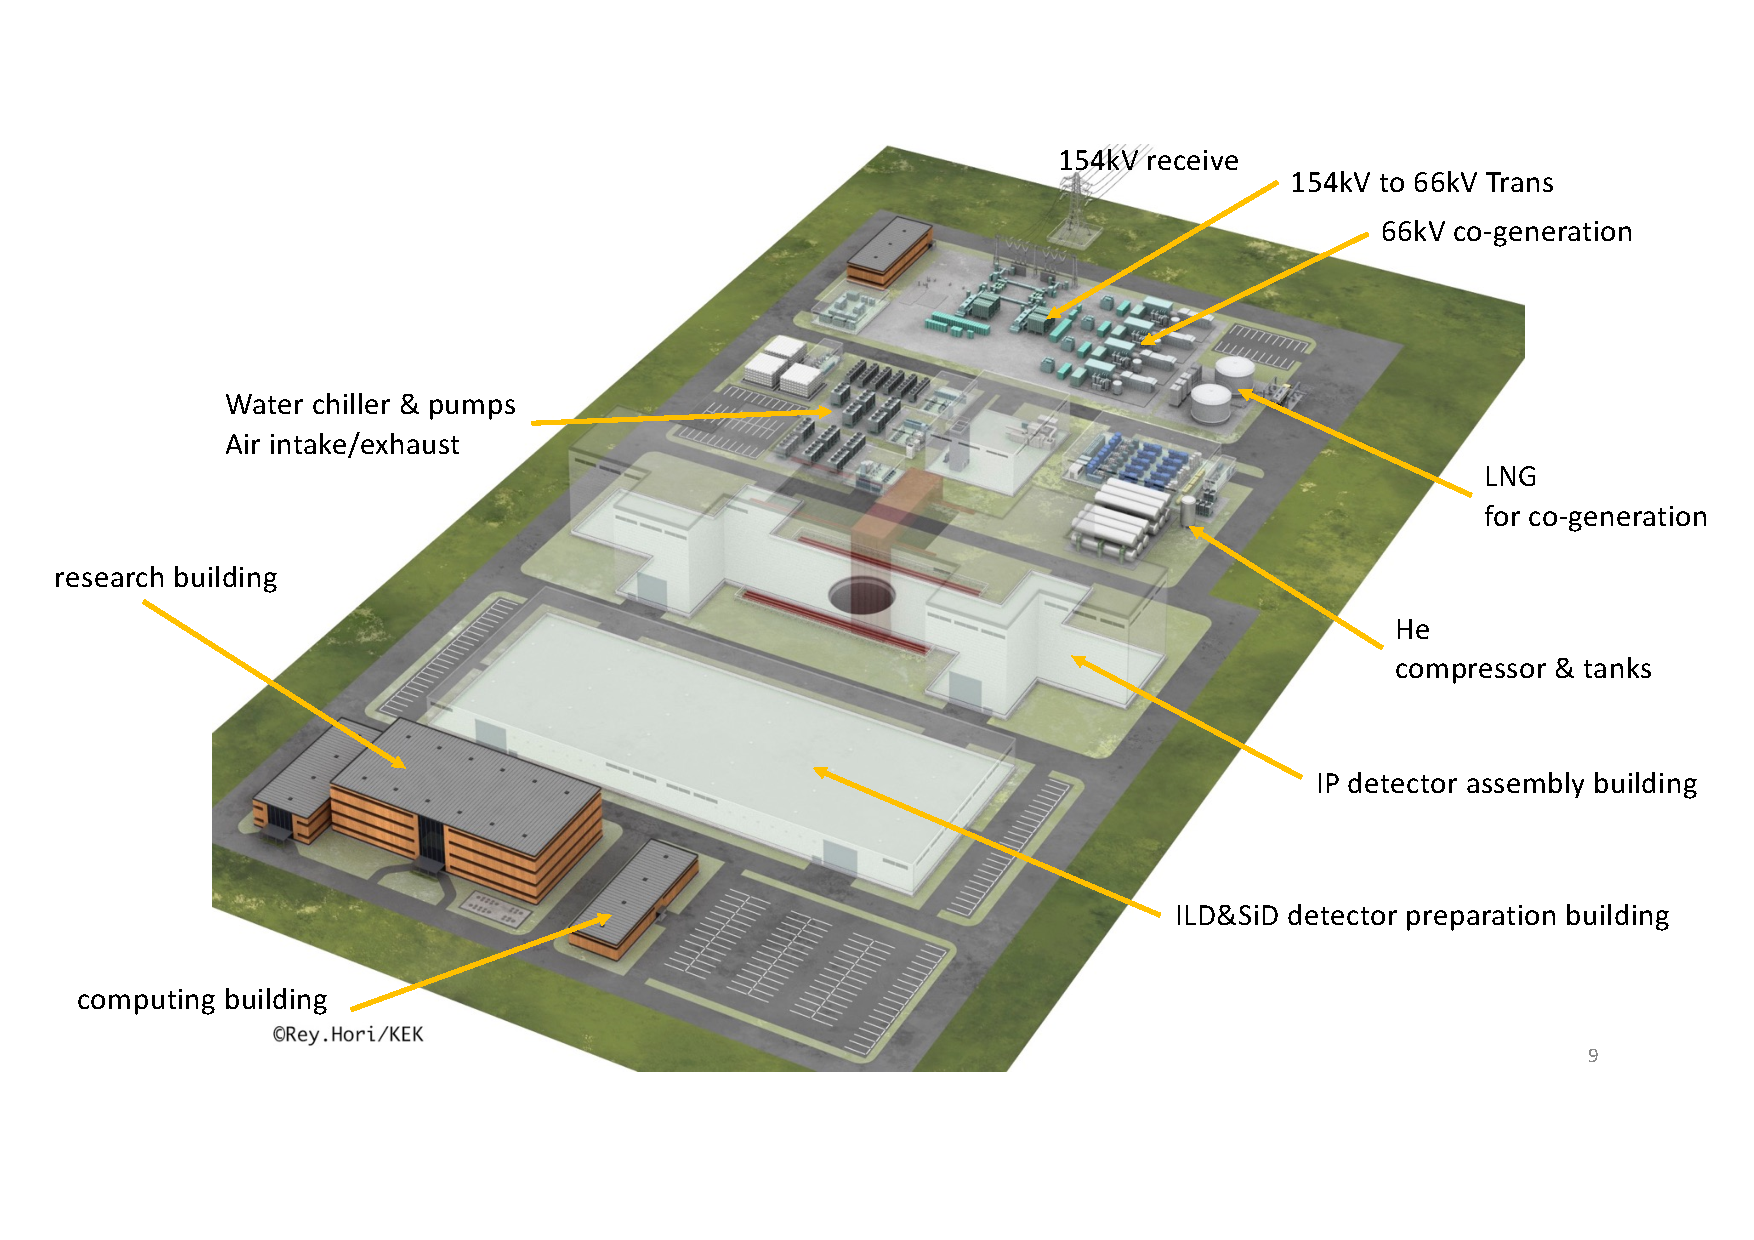
\includegraphics[width=1.1\hsize]{Integration/fig/Surface_Facilities.pdf}
\caption{\label{fig:integration:surface}Conceptual design (artist's view) of the surface facilities ("IP Campus") above the ILC interaction point~\cite{ild:bib:surface_facilities}. }
\end{figure}

The underground experimental hall is about 100~m below the surface and hosts two experiments, ILD and SiD, in a "push-pull" arrangement where both detectors share the same interaction region (c.f.~figure~\ref{fig:integration:underground}). The detectors are installed on movable platforms and can be rolled into or out of the beam line within a few hours. They can be opened and maintained in their parking positions. Access to the underground hall is provided by two vertical shafts and an access tunnel that allows for vehicles to drive directly into the underground area~\ref{fig:integration:access}.

\begin{figure}[h!]
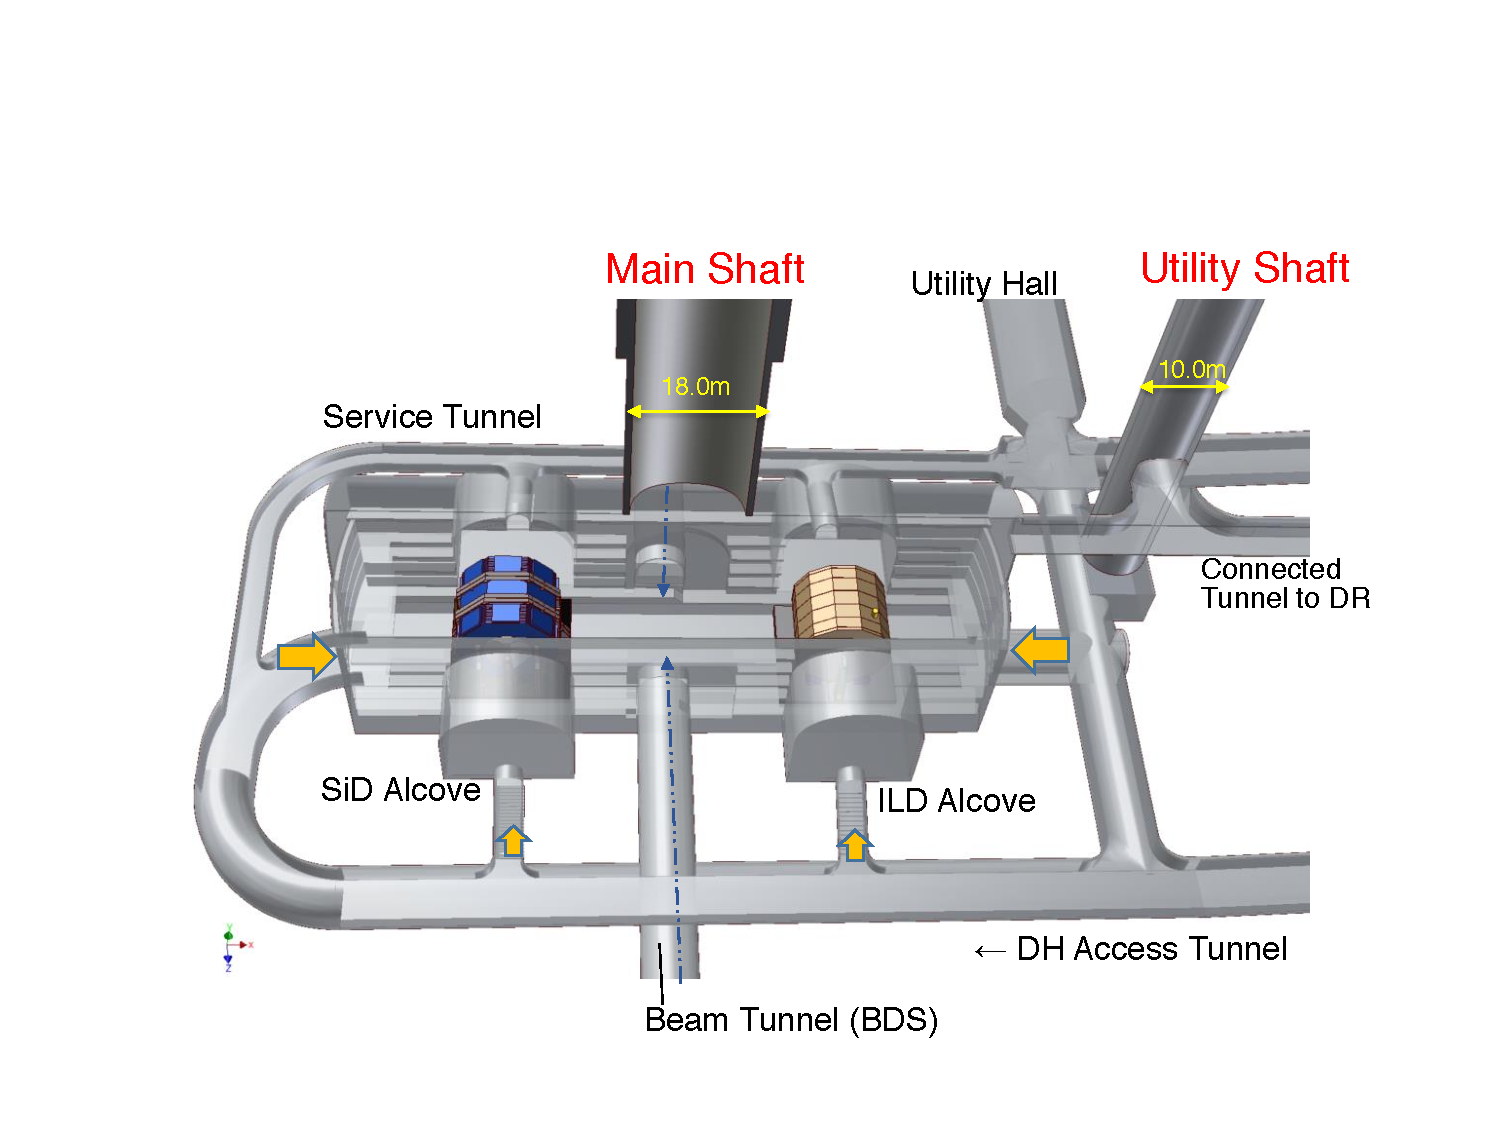
\includegraphics[width=1.0\hsize]{Integration/fig/Underground_Facilities.pdf}
\caption{\label{fig:integration:underground}Underground facilities with the detector hall, ILD and SiD in push-pull configuration, access tunnels and shafts~\cite{ild:bib:underground_facilities}. }
\end{figure}


\begin{figure}[h!]
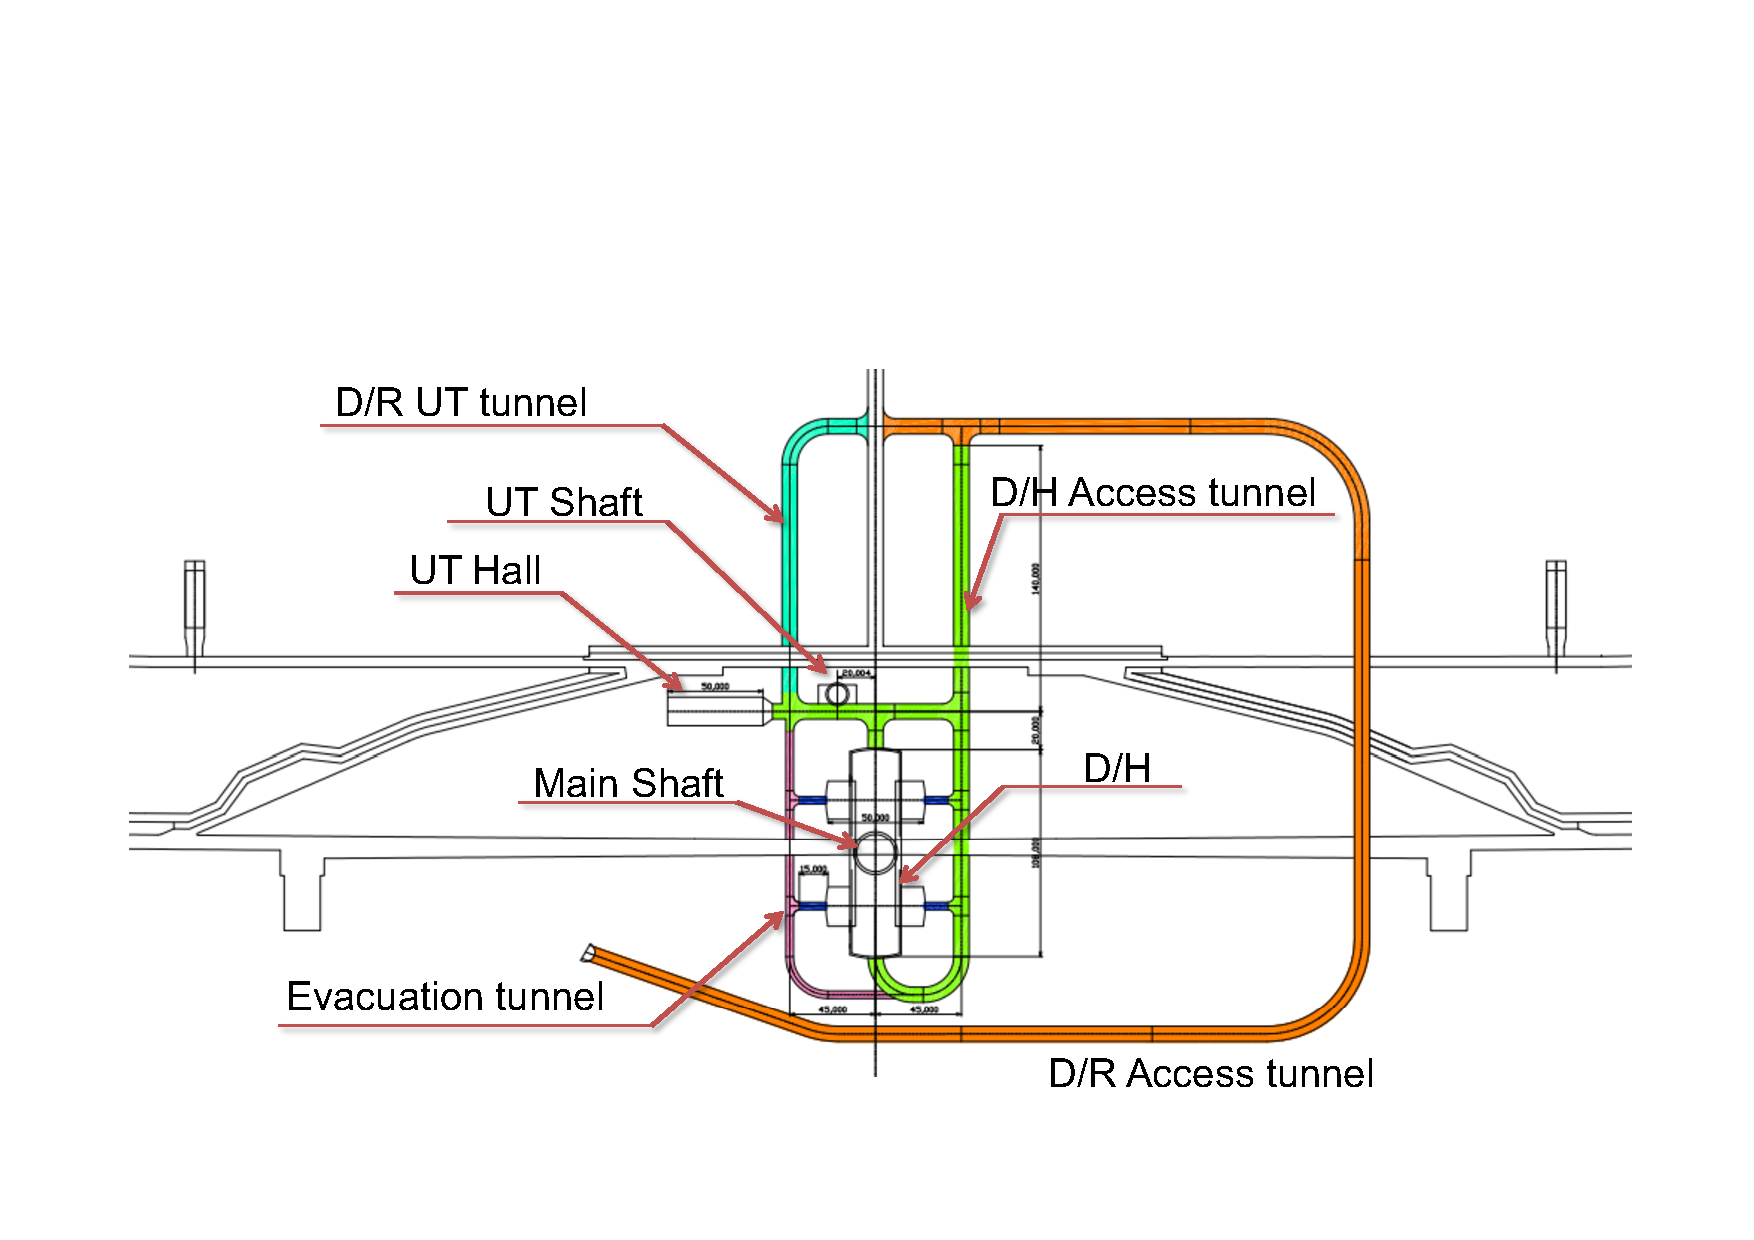
\includegraphics[width=1.0\hsize]{Integration/fig/Access.pdf}
\caption{\label{fig:integration:access}Access to the underground infrastructure is provided by two shafts, main shaft and utility (UT) shaft, and a system of access tunnels~\cite{ild:bib:Access} that serve the detector hall (DH) as well as the damping rings (DR). }
\end{figure}
%\vspace{2cm}

\subsection{Detector Utilities and Cavern Ancillary Services}
%\writer{Yasuhiro Sugimoto}{1}

%Summary of ancillary services from subdetectors in the cavern and on surface, as it will result from subdetector information to be provided in 
%Yasuhiro's excel file.

%ILD overall wish for utility space
%on the platform, the service gallery 
%and the service cavern.
In order to operate the ILD detector in the underground detector cavern, electricity, cooling water and other services have to be supplied from surface facilities. Though conceptual designs existed at the time of the DBD, more detailed knowledge about the requirements from the detector exists by now and should lead to an optimisation of the facilities layout and locations.


\subsubsection{Service Locations}
\label{ild:sec:service_locations}

There are several possible locations for detector services: on the detector platform, on service galleries on the wall of the detector hall, in dedicated utility/service caverns, and on surface. A possible configuration is shown in Figure~\ref{fig:integration:services}.
It is assumed that large or noisy apparatus such as transformers (6.6~kV$\rightarrow$400/200/100~V), heat exchangers and pumps for cooling water, sub-detector cooling plants, etc. should be located in the utility/service cavern. Cryogenic plant for the QF1 magnet is also supposed to be located in the utility/service cavern.

The utility/service cavern should be relatively close to the detector, but well isolated from the detector hall  regarding the noise, vibration, and radiation. Design of the facilities including caverns (CFS) for detector utilities/services has to be made based on requirements from the detector side. In order to clarify the requirements, a rough estimation on the ILD needs in electricity, cooling water, and space has been made (c.f. section~\ref{ild:sec:power}). 

The Design of the utility/service cavern is not fixed yet. In the baseline design (TDR-modified), the utility/service cavern has a dead-end as shown in Figure~\ref{fig:integration:access} (UT Hall in this figure). In addition, this cavern is supposed to be used for both detectors and accelerators, and does not have enough space for the estimated ILD needs. 
%Another proposal was made by a study team in Tohoku erea~\cite{ild:bib:tohokuutilitydesign}. In this design, the detector hall was extended by 25~m to be used for accelerator utilities, and the utility shaft is connected to this extended part. This design does not take detector utilities into account, and not acceptable for detectors. 
ILD proposes another design as shown in Figure~\ref{fig:integration:USC}. In this design, there are three utility/service caverns for accelerator, ILD, and SiD, respectively. The size of a detector utility/service cavern of 12~m$\times$34~m with two floors would be large enough for one detector.   Figure~\ref{fig:integration:services} is drawn assuming this utility/service cavern design.

\begin{figure}[h!]
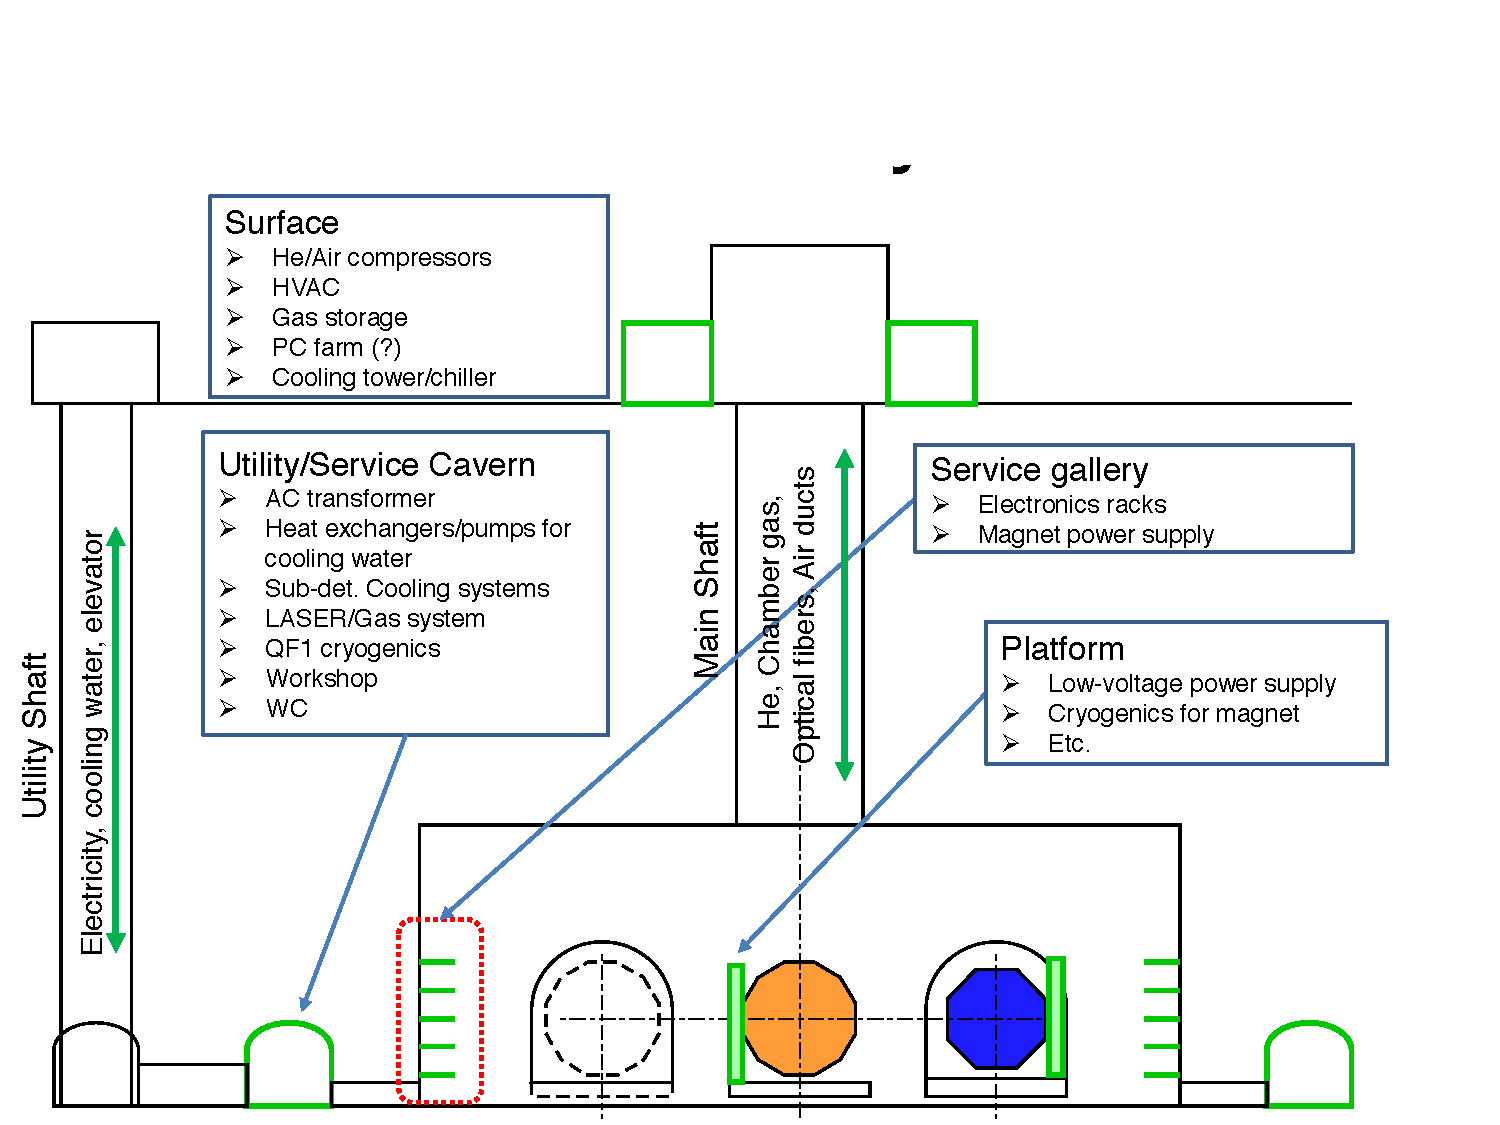
\includegraphics[width=1.0\hsize]{Integration/fig/Services.pdf}
\caption{\label{fig:integration:services}Schematic drawing of the possible locations for detector services. The Utility/Service cavern for the detector is proposed but not yet implemented into the ILC baseline design~\cite{ild:bib:services}. }
\end{figure}

\begin{figure}[h!]
\centering
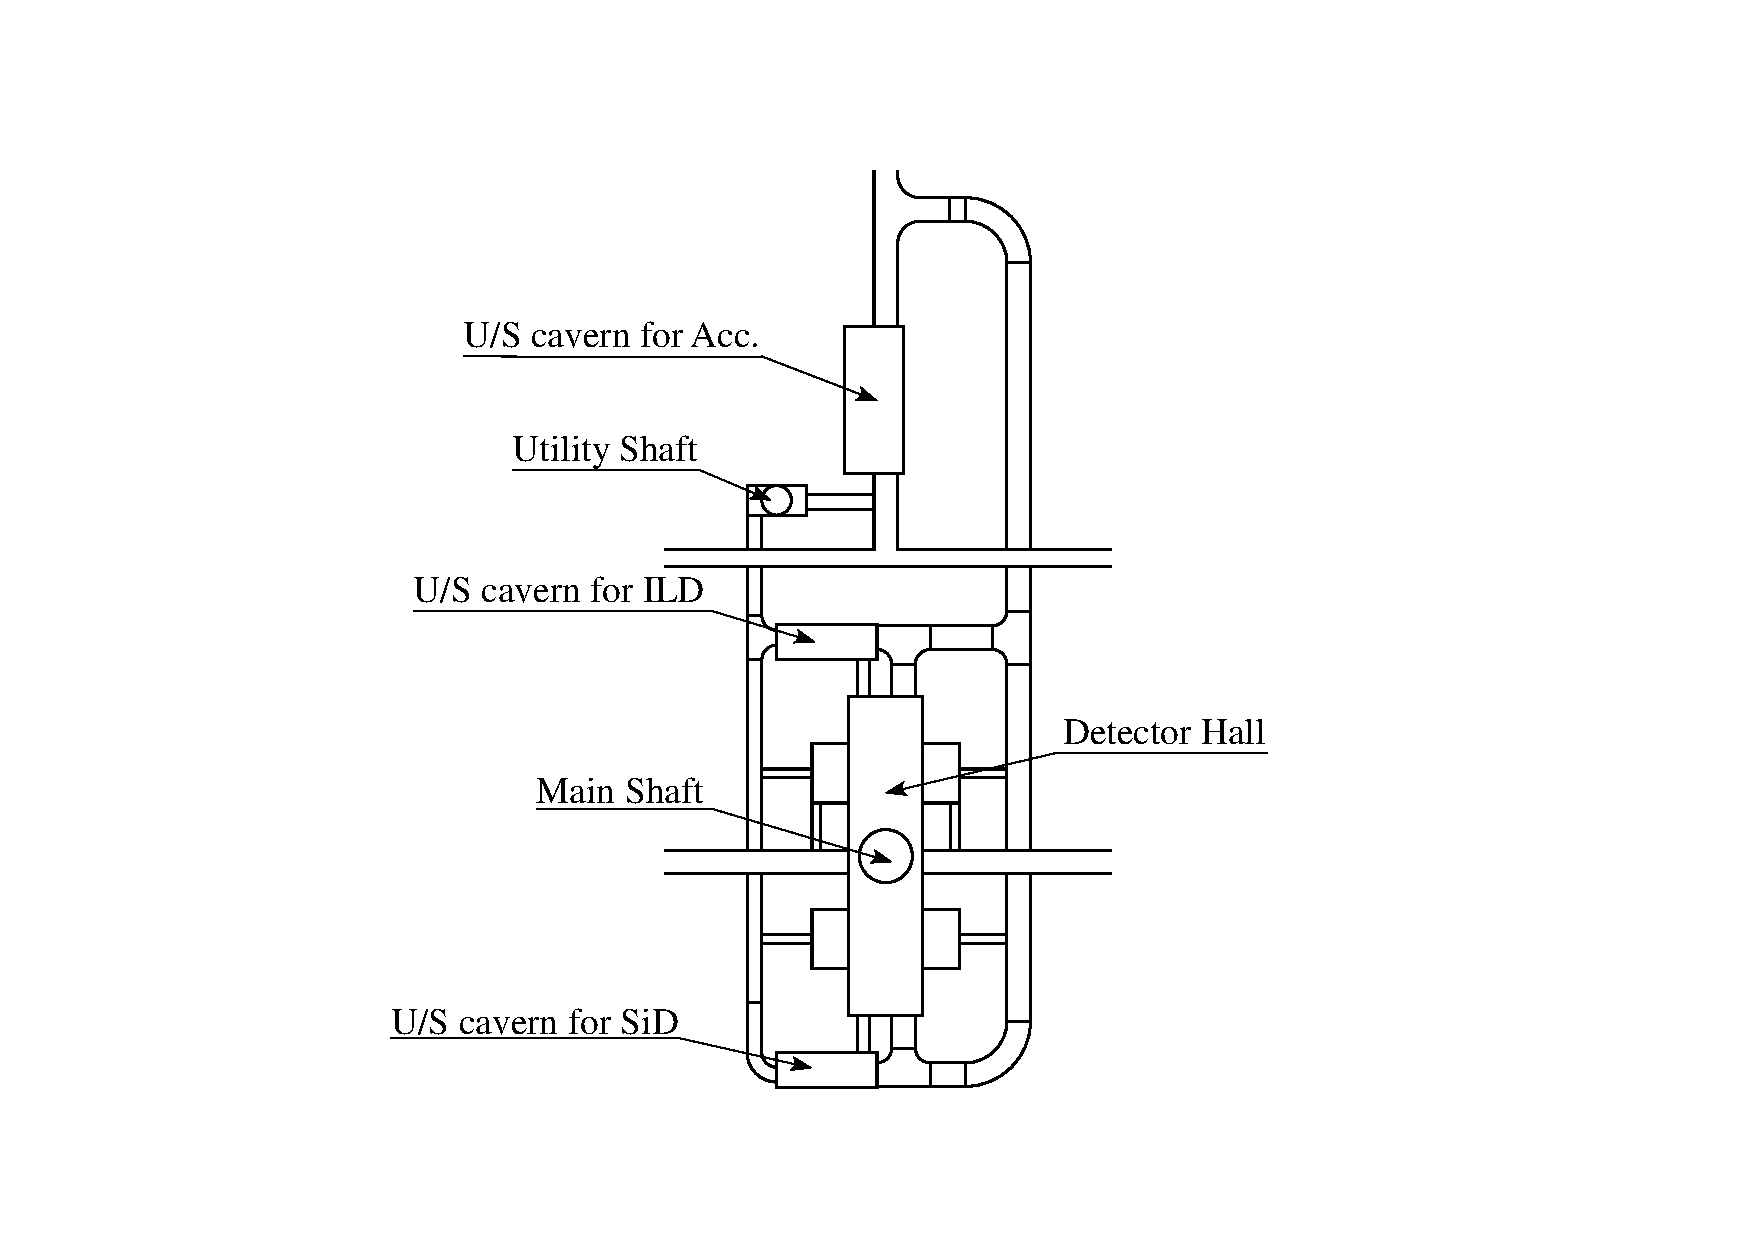
\includegraphics[width=0.5\hsize]{Integration/fig/USC.pdf}
\caption{\label{fig:integration:USC}A possible design of Utility/Service caverns. }
\end{figure}

\subsubsection{Power Consumption and Cooling Requirements}
\label{ild:sec:power}
The requirements for power and cooling at ILD have been studied in a bottom-up approach where the current information from all detector components has been assembled and cross-checked.

A tentative estimation of the power consumption in the detector hall and surface facilities for ILD is listed in Table~\ref{tab:integration:power}. The total power consumption in the underground caverns is about 1~MW, dominated by the ILD solenoid and the machine components associated to the detector. 

The cooling water which is necessary for extracting the power consumption is shown in Table~\ref{tab:integration:cooling}.
Distribution of the underground power is visualized in Figure~\ref{fig:integration:power}. It can be seen that the fraction of the power consumption that is coming from the sub-detectors is small.

\begin{table}[htb]
    \centering
    \begin{tabular}{l|l|c|c|c|c}
       \multicolumn{2}{l|}{{\bf Item}} & {\bf Power} &\multicolumn{3}{c}{ } \\ \hline
        \multirow{3}{*}{QD0/QF1/Crab Cavity} & Power Supply  & 150 & \multicolumn{3}{l}{ } \\
                            & Cold Box      & 150 & \multicolumn{3}{l}{ } \\
                            & He Compressor & 300 & \multicolumn{3}{l}{on surface}\\ \hline
        \multirow{3}{*}{Detector Solenoid} & Power Supply  & 250 & \multicolumn{3}{l}{ } \\
                            & Cold Box      & 50 & \multicolumn{3}{l}{ } \\
                            & He Compressor & 500 & \multicolumn{3}{l}{on surface}\\ \hline                      
        \multirow{10}{*}{Subdetectors} & {\bf Total}  & {\bf 161} & {\bf Front-end Electr.} & {\bf Back-end Electr.} & {\bf Cooling}\\ \cline{2-6}
        & Muon  & 12 & 5 & 5  & 2 \\
        & HCAL  & 45.5 & 27.5 & 8 & 10 \\
        & ECAL  & 40 & 20 & 12 & 8 \\
        & VFS   & 9 & 2 & 5 & 2 \\
        & SET   & 9 & 2 & 5 & 2 \\
        & TPC   & 16.2 & 15 & - & 1.2 \\
        & SIT   & 8 & 1 & 5 & 2 \\
        & FTD   & 8 & 1 & 5 & 2 \\
        & VTX   & 13.5 & 2 & 1.5 & 10 \\\hline
        \multicolumn{2}{l|}{Computer Farm}& 1000 & \multicolumn{3}{l}{on surface}\\ \hline
        \multicolumn{2}{l|}{Water Pump}& 25 & \multicolumn{3}{l}{}\\ \hline
        \multicolumn{2}{l|}{HVAC}& 600 & \multicolumn{3}{l}{on surface}\\ \hline
        \multicolumn{2}{l|}{Lighting}& 25 & \multicolumn{3}{l}{}\\ \hline
        \multicolumn{2}{l|}{Air Compressor}& 50 & \multicolumn{3}{l}{on surface}\\ \hline
        \multicolumn{2}{l|}{Platform Mover}& 100 & \multicolumn{3}{l}{}\\ \hline
        \multirow{2}{*}{Cranes} & 3x5t & 21 & \multicolumn{3}{l}{}\\
        & 40t & 50 & \multicolumn{3}{l}{}\\ \hline
        \multicolumn{2}{l|}{{\bf TOTAL}}& {\bf 3432} & \multicolumn{3}{l}{}\\ \hline
        \multicolumn{2}{l|}{Underground}& 982 & \multicolumn{3}{l}{}\\ \hline
    \end{tabular}
    \caption{Breakdown of the power consumption estimates for the ILD detector and appended ILC components (in kW)~\cite{ild:bib:services}.}
    \label{tab:integration:power}
\end{table}

\begin{table}[]
    \centering
    \begin{tabular}{m{1.4cm}|m{1.7cm}|m{0.6cm}|m{0.6cm}|m{0.7cm}|m{0.6cm}|m{0.6cm}|m{0.7cm}|m{0.6cm}|m{0.6cm}|m{0.7cm}}
    \multicolumn{2}{m{1.4cm}|}{}& \multicolumn{3}{c|}{Chilled Water} & \multicolumn{3}{c|}{Low-conductive Water} & \multicolumn{3}{c}{Normal Water} \\ \hline
    \multicolumn{2}{m{1.4cm}|}{Item} & Heat (kW) & $\Delta$T (K) & Flow (l/min) & Heat (kW) & $\Delta$T (K) & Flow (l/min) & Heat (kW) & $\Delta$T (K) &Flow (l/min) \\ \hline
    \multirow{2}{1.4cm}{QD0/QF1/ Crab Cav.} & Power Supply & & & & 150 & 10 & 214 & & & \\
    & Cold Box & & & & 150 & 10 & 214 & & & \\\hline
    \multirow{2}{1.4cm}{Detector Solenoid} & Power Supply & & & & 250 & 10 & 357 & & & \\
    & Cold Box & & & & 50 & 10 & 71 & & & \\\hline
    \multirow{9}{1.4cm}{Subdetectors} & Muon & 12 & 5 & 34 & & & & & \\
    & HCAL & 45.5 & 5 & 130 & & & & & & \\
    & ECAL & 40 & 5 & 114 & & & & & & \\
    & VFS & 9 & 5 & 26 & & & & & & \\
    & SET & 9 & 5 & 26 & & & & & & \\
    & TPC & 3 & 5 & 5 & & & & 13 & 5 & 38\\
    & SIT & 8 & 5 & 23 & & & & & & \\
    & FTD & 8 & 5 & 23 & & & & & & \\
    & VTX & 13.5 & 5 & 39 & & & & & & \\\hline
    \multicolumn{2}{m{2cm}|}{Pump} & 11 & 5 & 31 & 11 & 10 & 16 & 3.7 & 5 & 11\\ \hline
    \multicolumn{2}{m{2cm}|}{AC Transformer} & 49 & 5 & 140 & & & & & & \\ \hline
    \multicolumn{2}{m{2cm}|}{{\bf Total}} & 208 & & 595 & 611 & & 873 & 17 & & 48 \\ \hline
    \multicolumn{2}{l|}{{\bf Total Chilled Water}} & \multicolumn{3}{r|}{{\bf 595}} & \multicolumn{6}{r}{}\\ \hline
    \multicolumn{2}{l|}{{\bf Total Normal Temp. Water}} & \multicolumn{3}{r|}{} & \multicolumn{6}{r}{{\bf 921}}\\ \hline

    \end{tabular}
    \caption{Breakdown of the cooling water requirement estimates for ILD and appended ILC components~\cite{ild:bib:services}.}
    \label{tab:integration:cooling}
\end{table}

\begin{figure}[h!]
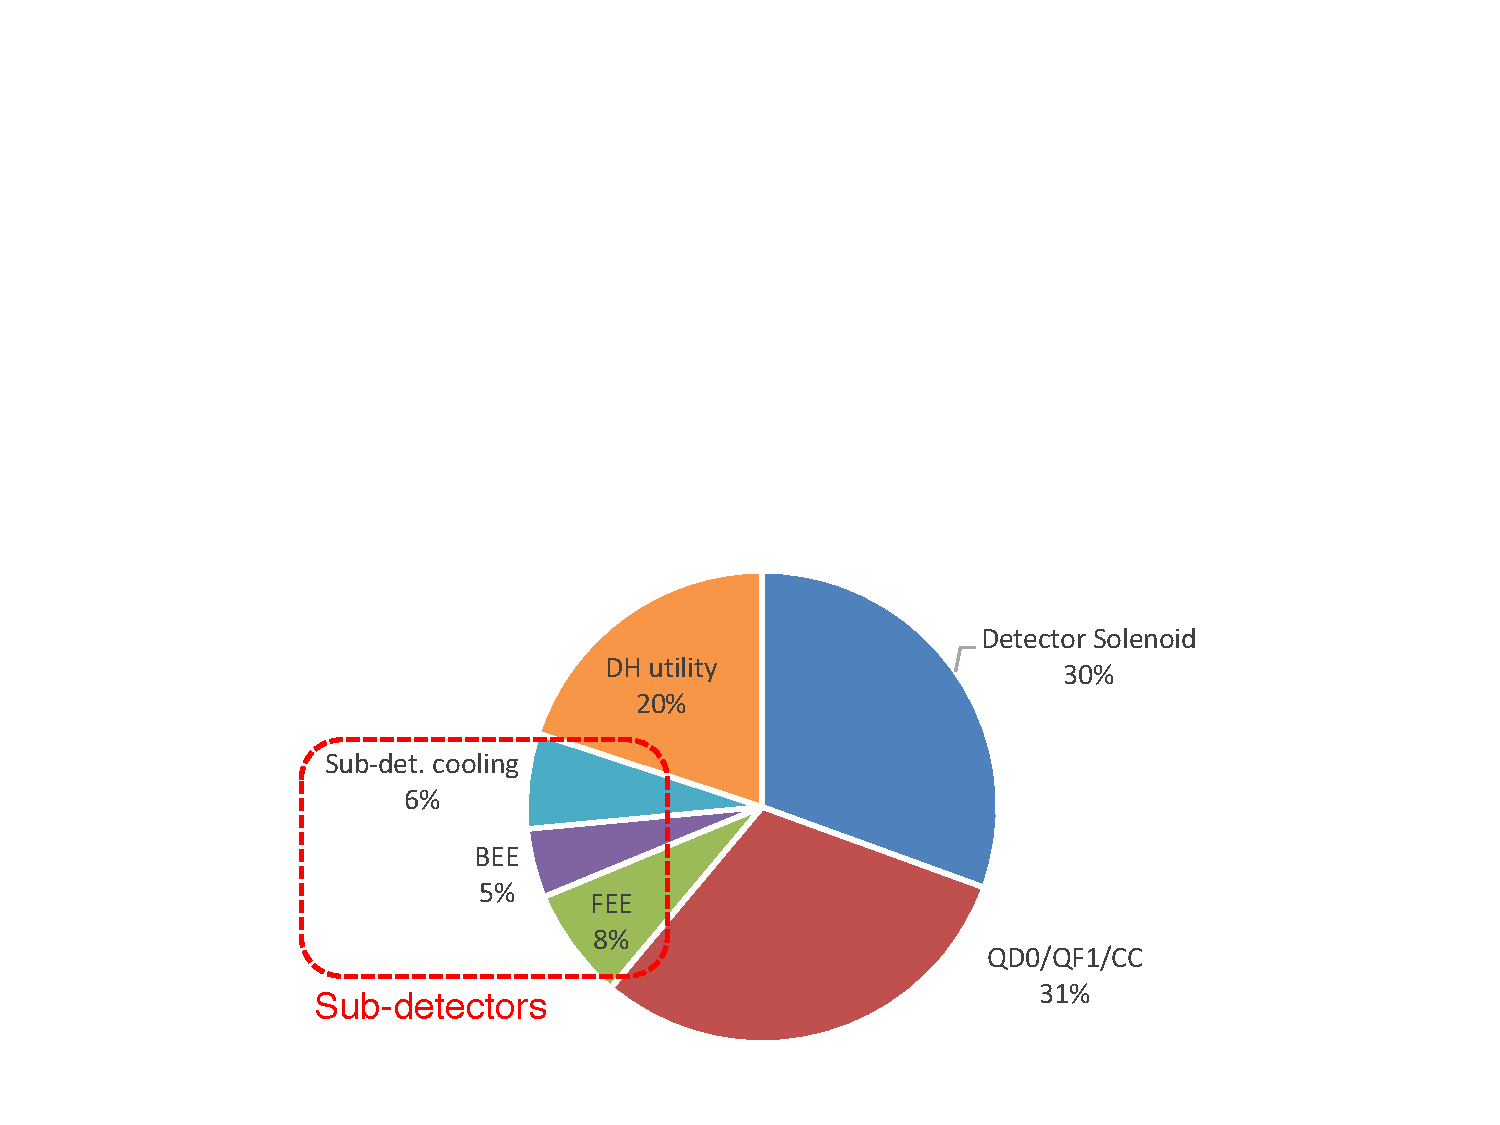
\includegraphics[width=0.7\hsize]{Integration/fig/Power.pdf}
\caption{\label{fig:integration:power}Distribution of the underground power consumption for ILD~\cite{ild:bib:services}. While the detector solenoid, the machine elements (magnets QD0/QF1 and the crab cavity system CC) use the major part of the power, the detector hall (DH) utilities and the sub-detectors cooling, back- and front-end electronics (BEE, FEE) contribute less. The total power consumption sums up to about 1~MW.}
\end{figure}
\vspace{2cm}
\FloatBarrier

\subsection{Access and Assembly}
\label{ild:sec:access}
The Kitakami site of the ILC is located in a mountainous and rural area, only accessible by road~(c.f.~figure~\ref{ild:fig:ilc_site}). The nearest port, Kesennuma, is about 40~km away on the Pacific coast. All ILD parts need to be shipped via the central access roads into the mountains. Typically, street transport in Japan is limited to trucks with up to 25~t of mass (including the weight of the truck itself). The total mass of ILD is of about 15,500~t, posing a specific challenge for the logistics infrastructure. Heavy-load transports of up to 70~t loads are possible in exceptional cases. For the transport of the ILD solenoid modules, this option is under study~(c.f.~figure~\ref{ILD:fig:magnet_transport}).

The heaviest parts of ILD are the yoke rings. They need to be assembled on-site from pre-fabricated iron blocks. Figure~\ref{fig:integration:yoke_assembly} shows three options that are under study for the procedures. If a remote campus close to the interaction region could be made available, with a dedicated reinforced street in-between, then the pre-fabricated iron slabs from the factory could be assembled into blocks of up to 200~t there. The blocks could then be transported via the dedicated road to the interaction region for assembly of the yoke rings. Another option would be the construction of a pre-assembly hall at the interaction region. The construction of the iron block could then take place there, in vicinity of the detector assembly hall and therefore a reduced transportation problem. A remote area would still be useful as storage space.
\begin{figure}[h!]
\centering
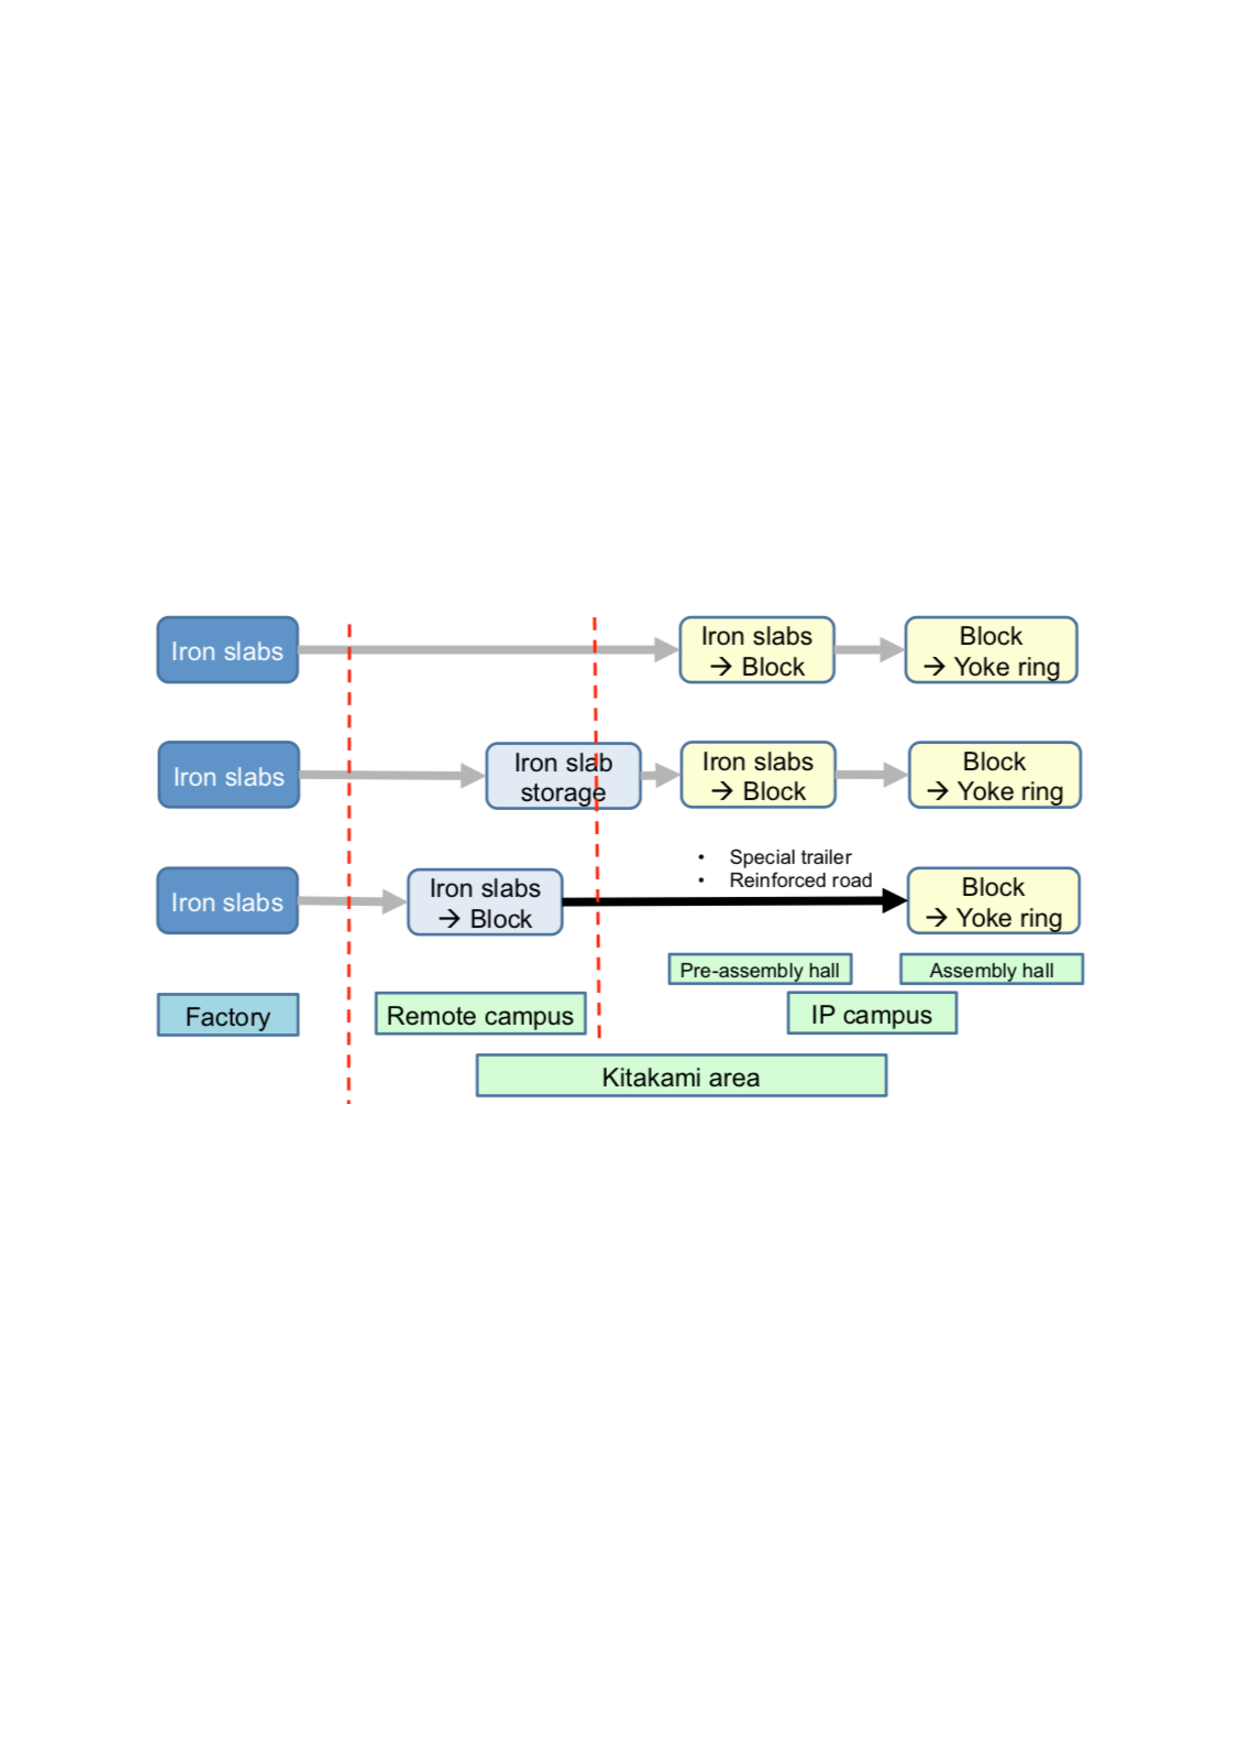
\includegraphics[width=0.8\hsize]{Integration/fig/yoke_assembly.pdf}
\caption{\label{fig:integration:yoke_assembly}Options under study for the (pre)assembly of the ILD iron return yoke~\cite{ild:bib:ejade_mdi}.}
\end{figure}

Figure~\ref{fig:integration:surface} shows a conceptual layout of the surface installations above the interaction region. The central detector assembly hall serves both detectors, SiD and ILD, and is located above the central access shaft to the underground areas (compare figure~\ref{fig:integration:underground}). A pre-assembly building for SiD and ILD is located right next to it. Heavy and large parts, like the ILD yoke blocks, could be assembled in the pre-assembly area before they are moved to the central assembly hall for the installation of the yoke rings.
%\begin{figure}[p]
%\centering
%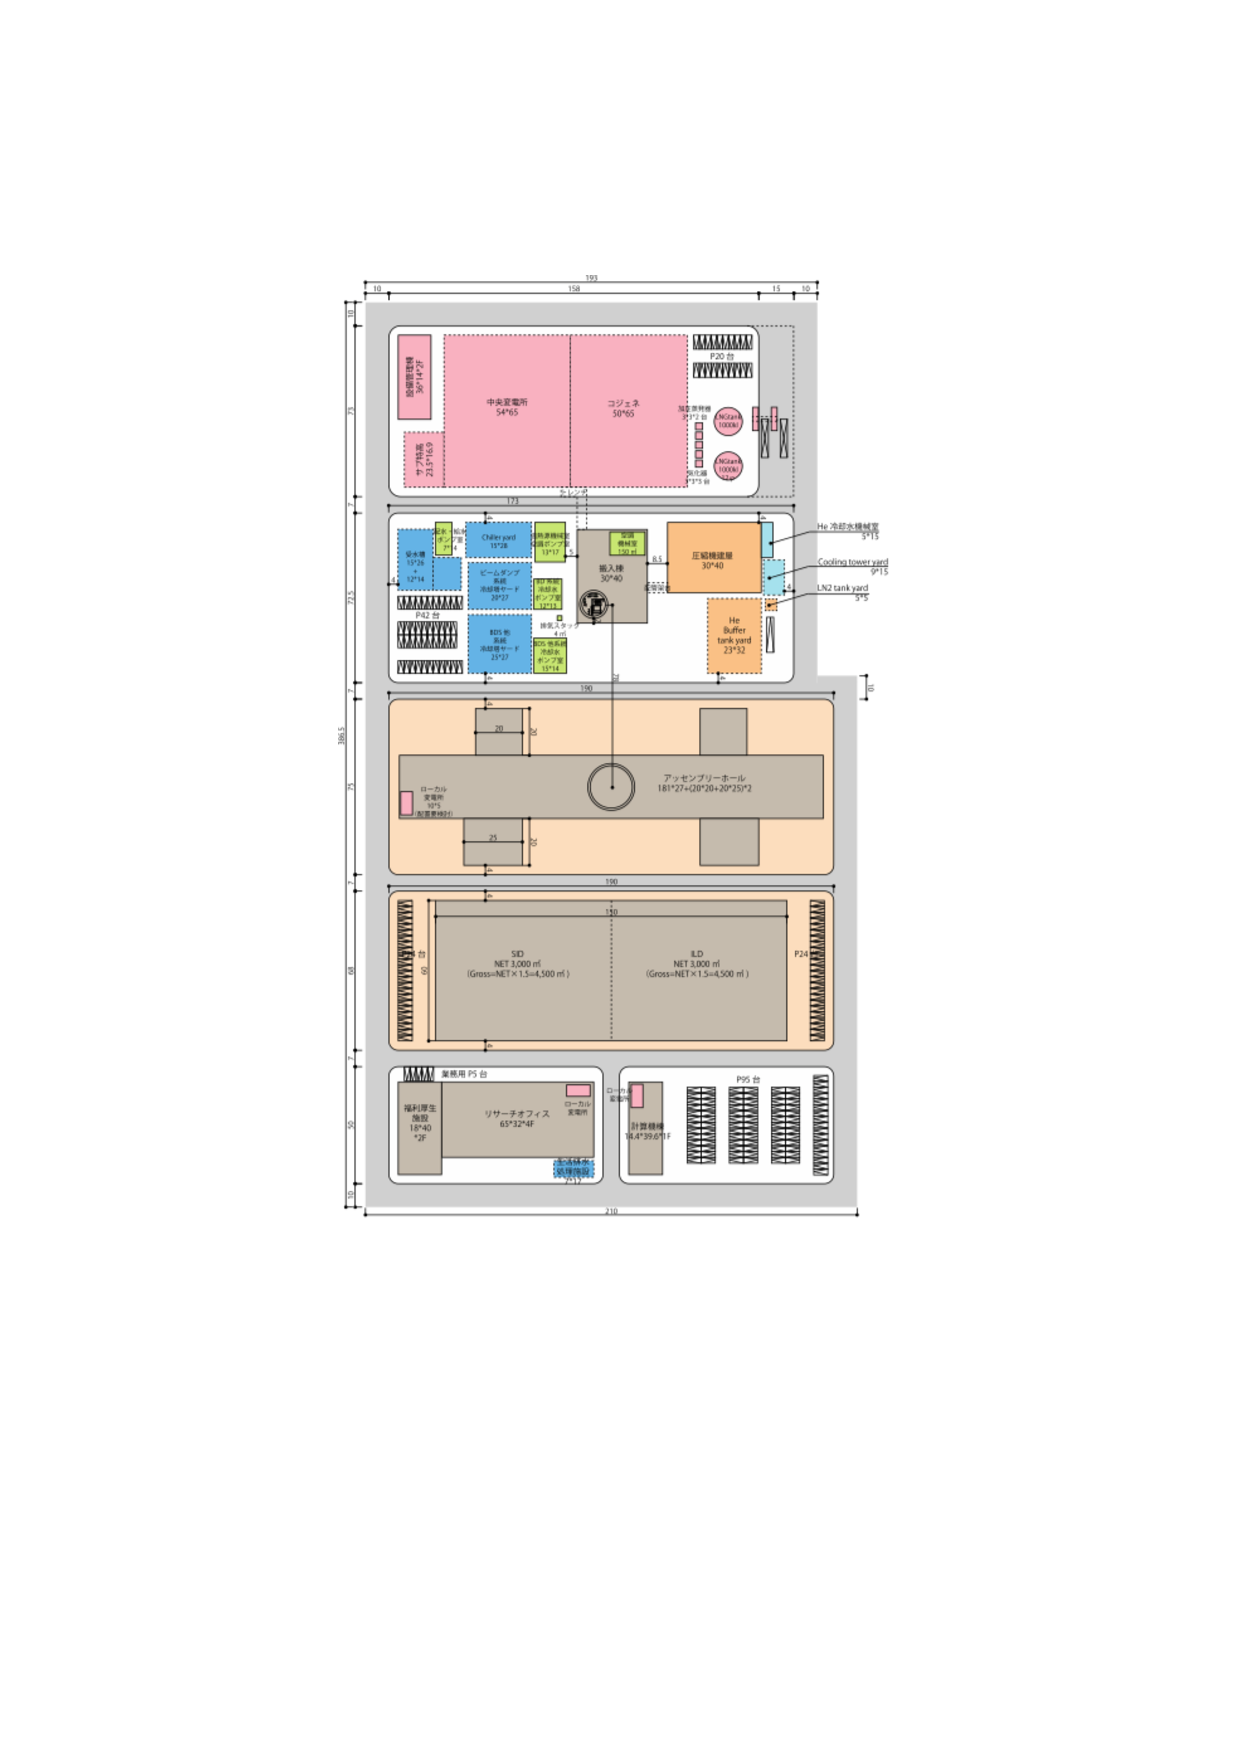
\includegraphics[width=0.8\hsize]{Integration/fig/interaction_area.pdf}
%\caption{\label{fig:integration:interaction_area}Conceptual design of the %interaction area surface installations with the detector assembly hall over %the large shaft in the middle and with a dedicated detector pre-assembly %building next to it~\cite{ild:bib:ejade_mdi}.}
%\end{figure}

A survey has been done within ILD to assemble the requirements of the sub-detectors on assembly, storage and on-site testing space. Figure~\ref{fig:integration:assembly_space} shows the results from SDHCAL, TPC and SiECAL (barrel and endcap). Though the information is at a very conceptual level, it serves as valuable input for the planners of the interaction region surface installations that need to be accommodated in the Kitakami mountains.
\begin{figure}[h!]
\centering
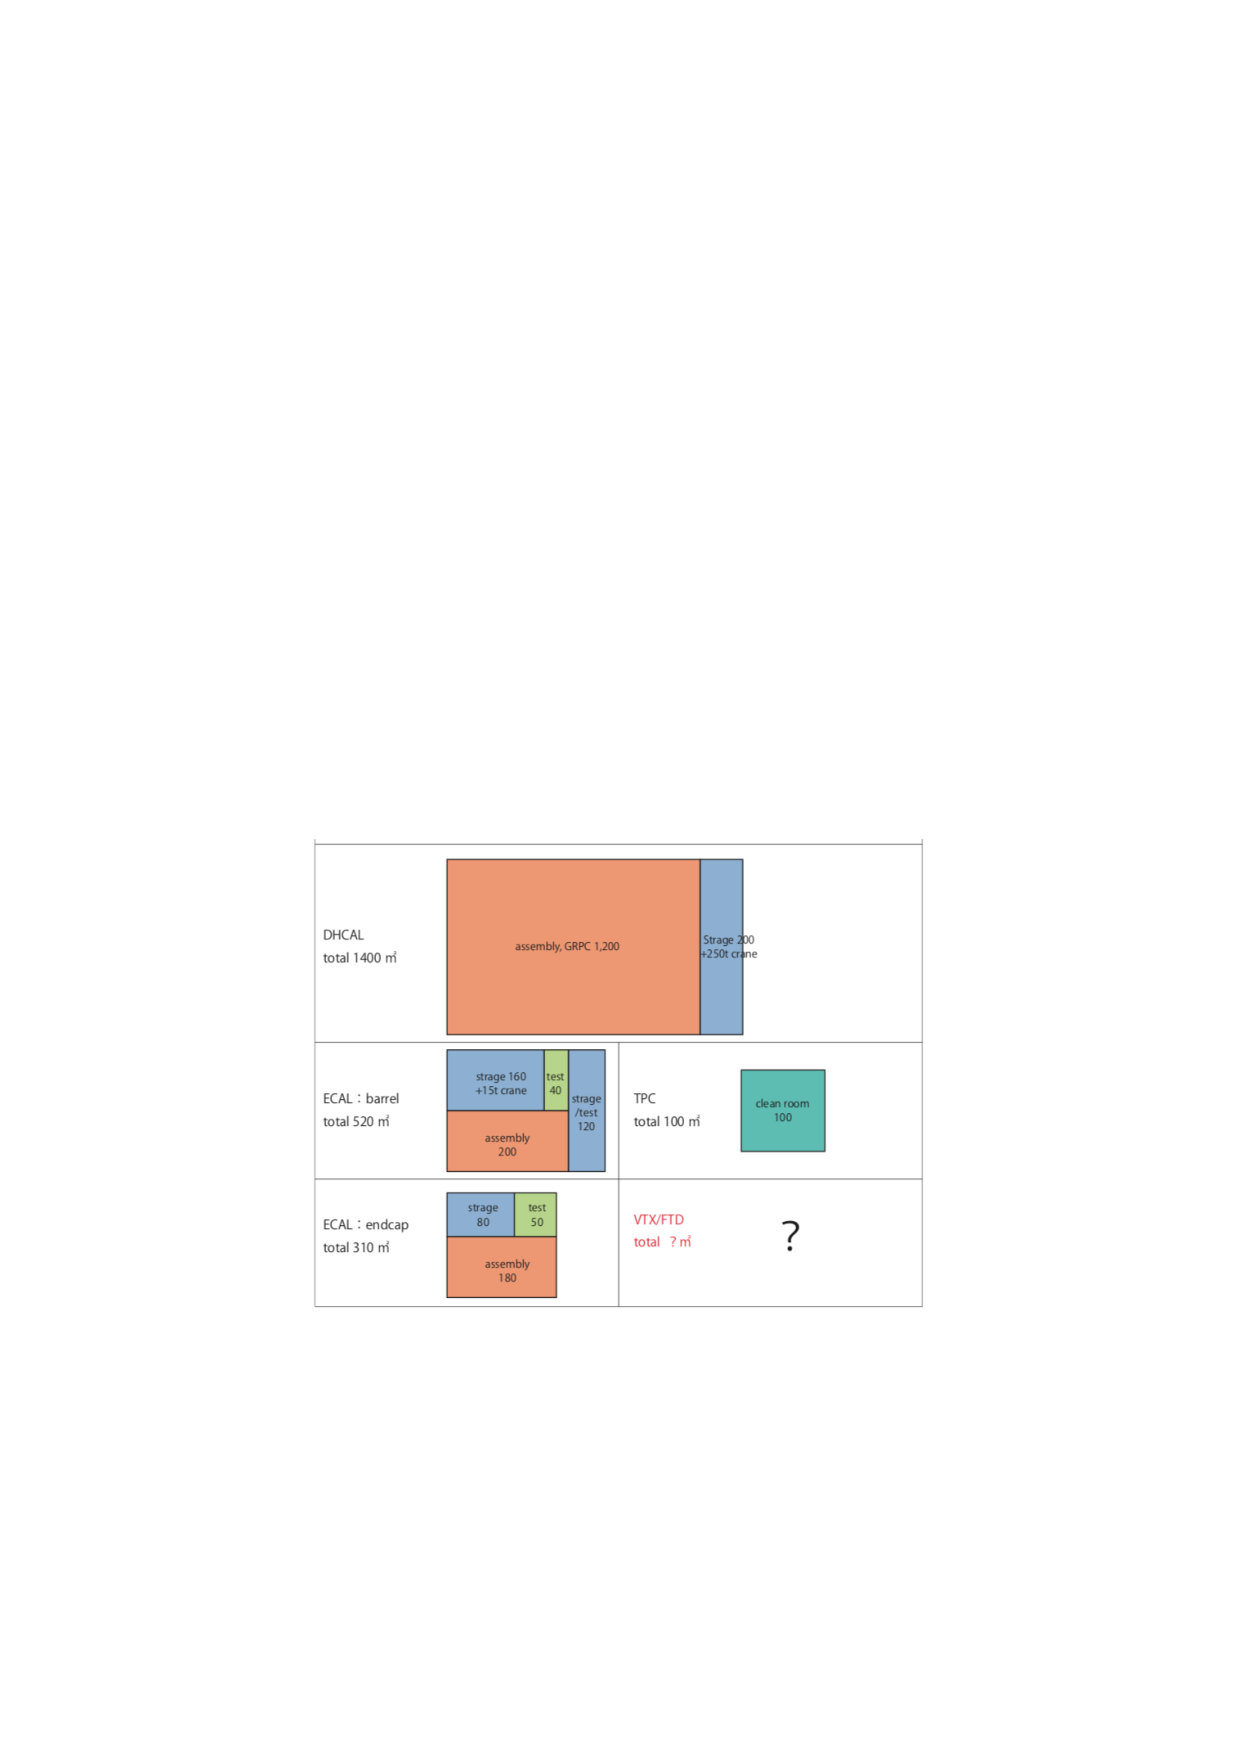
\includegraphics[width=0.8\hsize]{Integration/fig/assembly_space_survey.pdf}
\caption{\label{fig:integration:assembly_space}Result of a subdetector survey on assembly space requirements~\cite{ild:bib:ejade_mdi}.}
\end{figure}

The final assembly of ILD and SiD should happen above ground in the central detector assembly hall. The major parts, the SiD barrel detector and the ILD yoke rings, have masses of up to 4500~t and will be lowered through the central access shaft into the underground areas with the help of a gantry crane. A similar procedure has been followed for the CMS detector at CERN and was proven to be very efficient. Figure~\ref{fig:integration:gantry_crane} shows an artists view of the SiD barrel detector hanging from a gantry crane.
\begin{figure}[h!]
\centering
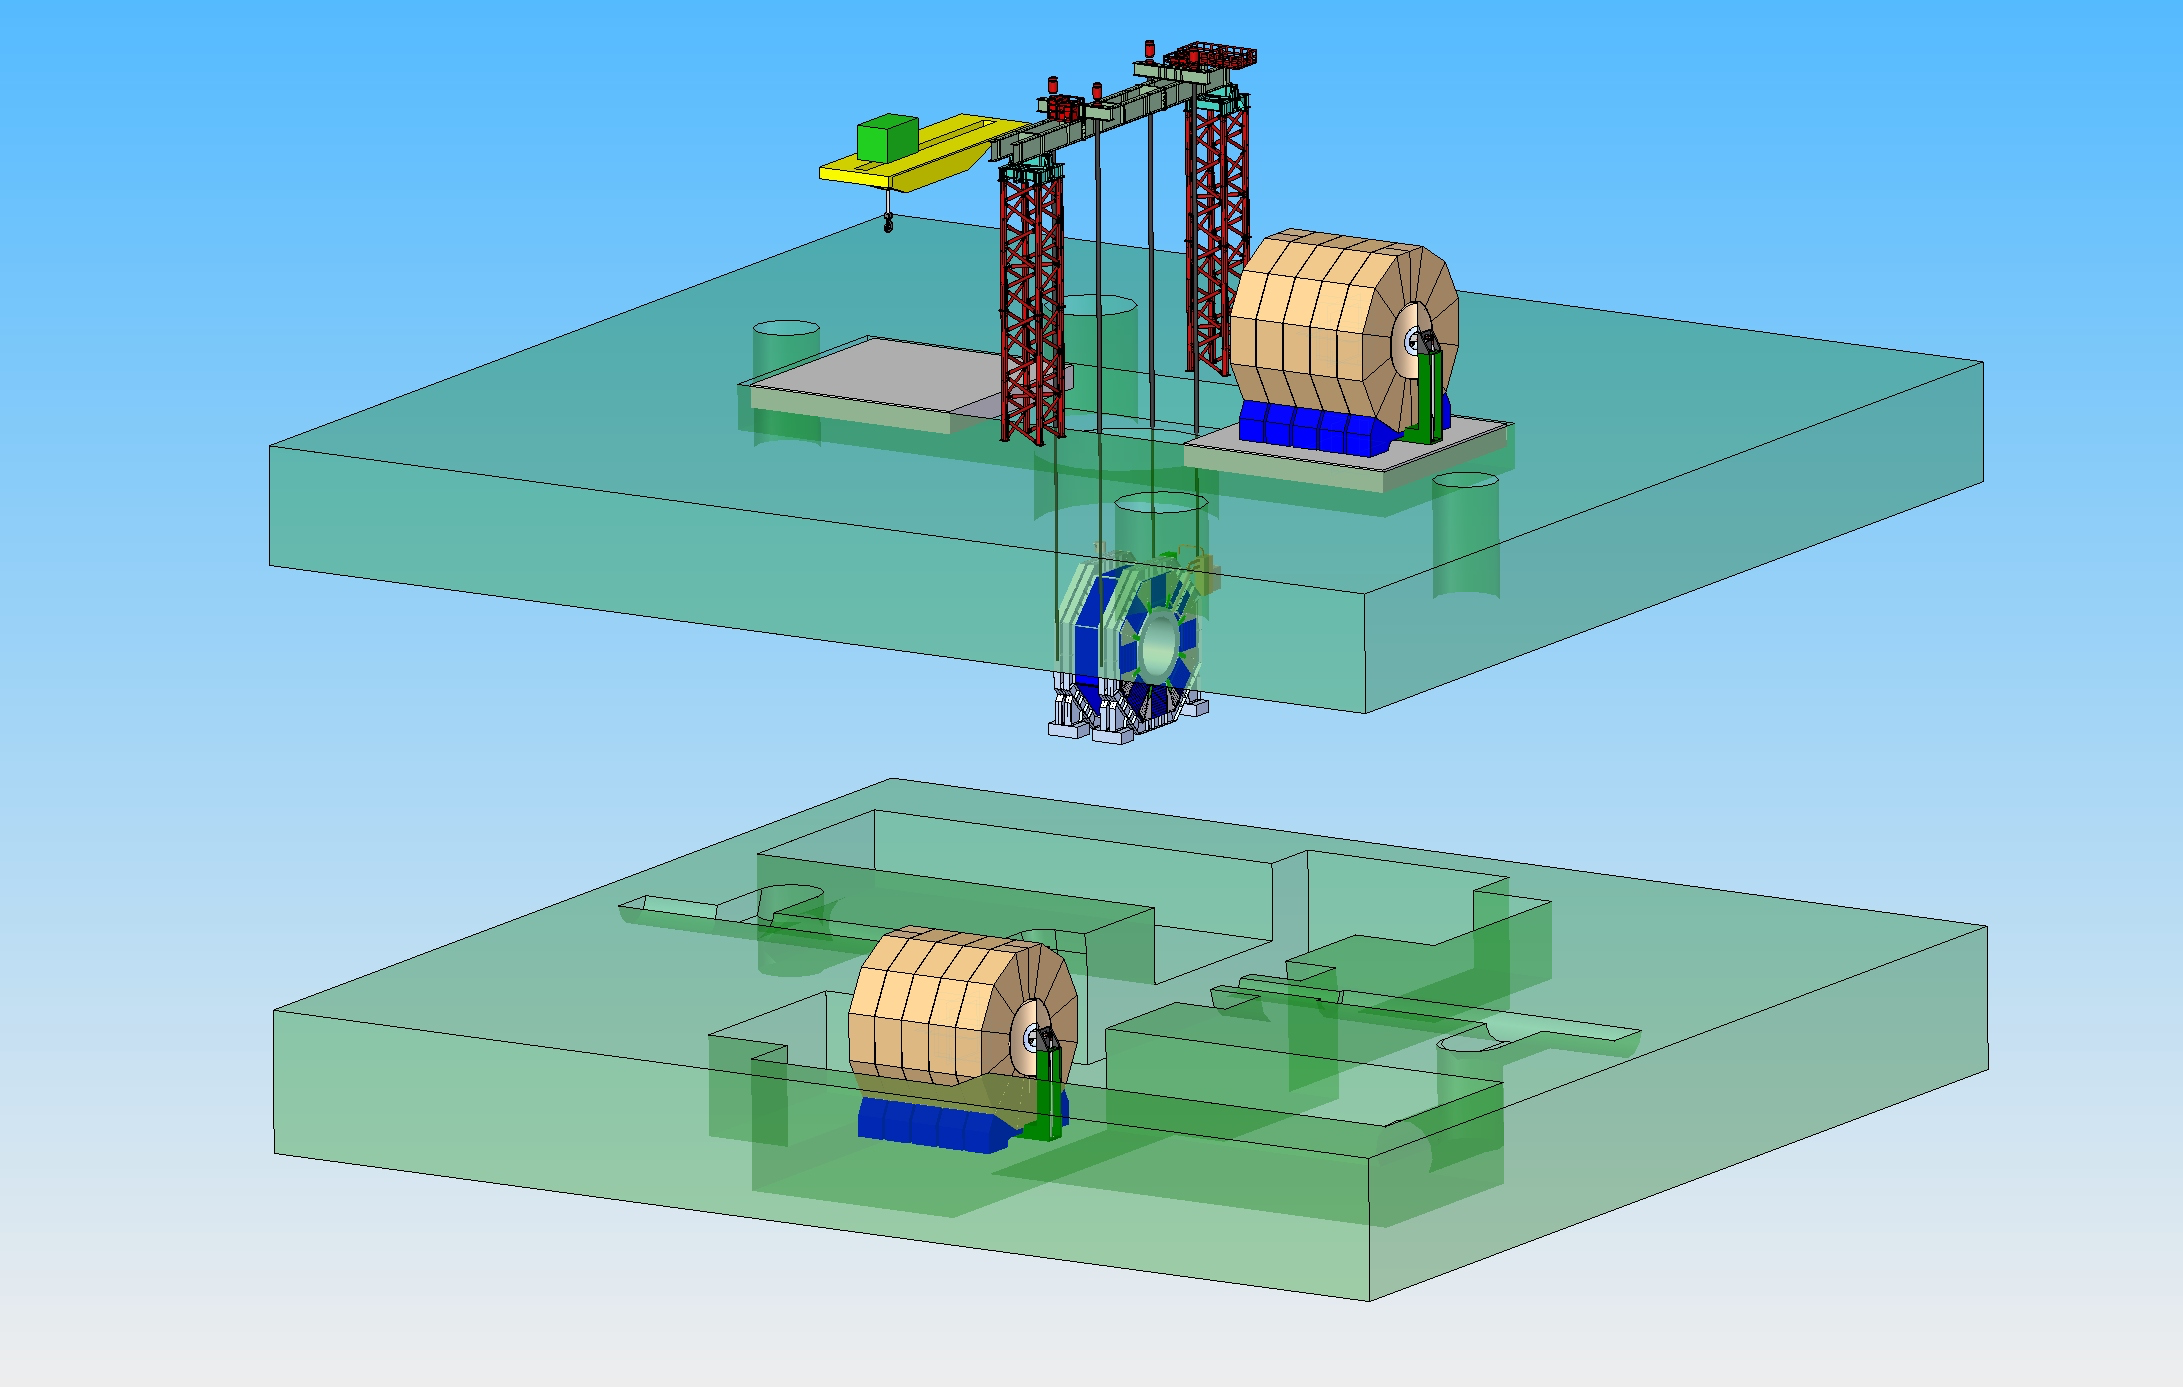
\includegraphics[width=0.8\hsize]{Integration/fig/gantry_crane.png}
\caption{\label{fig:integration:gantry_crane}Lowering of SiD and ILD main parts via the central shaft into the underground detector hall with the help of a heavy load gantry crane~\cite{ild:bib:gantry_crane}.}
\end{figure}

The main advantage of the CMS-style surface assembly of the detectors lies in the decoupled time lines for the construction of the machine and the detectors. In this case, the on-site assembly can start as soon as the surface buildings are ready while the underground excavations and constructions can carry on. Figure~\ref{fig:integration:assembly_timeline} shows a rough schedule for the detector construction.
\begin{figure}[h!]
\centering
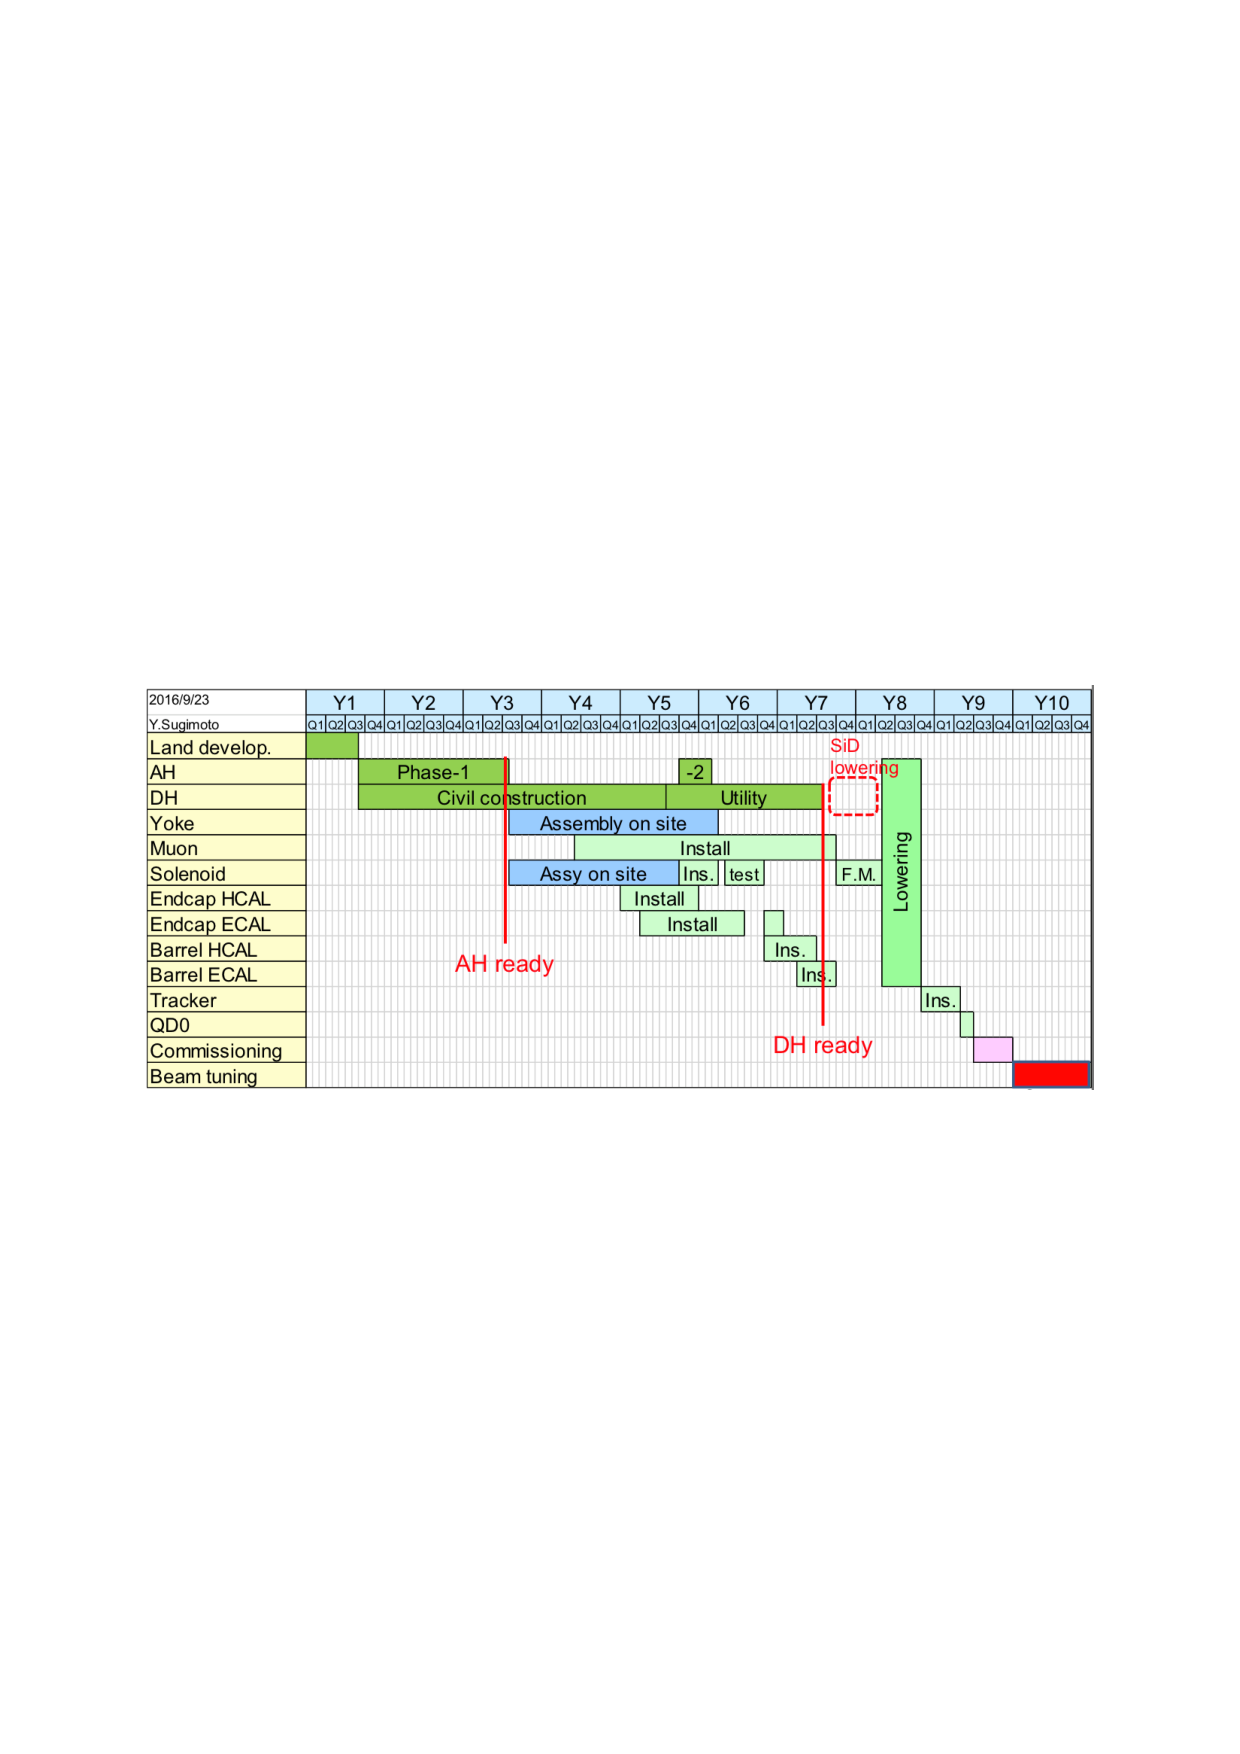
\includegraphics[width=0.8\hsize]{Integration/fig/assembly_timeline.pdf}
\caption{\label{fig:integration:assembly_timeline}Tentative timeline for the detector construction and assembly~\cite{ild:bib:ejade_mdi}.}
\end{figure}
On-site assembly can start 2.5~y after the ground breaking when the surface buildings are ready. The lowering of the large detector parts only takes place about one year before the commissioning of the machine would start. The total technical construction and assembly time is of about 9 years.